\section{Fluoreszenz}
\authors{Ole Simmering, Ailin Sigel}

Fluoreszenz ist die Emission von Energie in Form von Licht kurz nach der Anregung eines Systems \cite{Atkins2001}. Dabei wird das gesamte System zuerst vertikal in einen höheren elektronischen Zustand angeregt (siehe Abbildung \ref{fig:Energiegraphen der elektronischen Zustände bei der Fluoreszenz}) und begibt sich dann zunächst strahlungslos in den Schwingungsgrundzustand des angeregten elektronischen Zustandes (siehe Abbildung \ref{fig:Energieniveaus der Fluoreszenz}). Nun fällt das System in den elektronischen Grundzustand zurück. Hierbei wird weniger Energie in Form von Licht frei, als vorher absorbiert wurde, um das System in den angeregten Zustand zu bringen.

\begin{dsafigure}
	\centering
	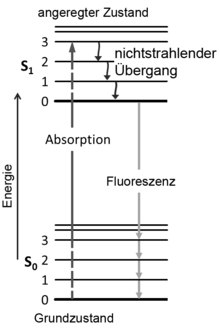
\includegraphics[width=4cm]{Fluoreszenz_Energieniveaus.png}
	\label{fig:Energieniveaus der Fluoreszenz}
	\caption{Energieniveauschema der Fluoreszenz \cite{wikiJablonskiDiagramm}.}
\end{dsafigure}

Es gilt für das Potential zweier gebundener Kerne: Bei sehr großer Nähe der Kerne läuft das Potential gen unendlich. Bei hinreichendem Abstand erreicht das Potential ein Minimum und nähert sich bei größerem Abstand einem Energiewert an (siehe Abbildung \ref{fig:Energiegraphen der elektronischen Zustände bei der Fluoreszenz}).

\begin{dsafigure}
	\centering
	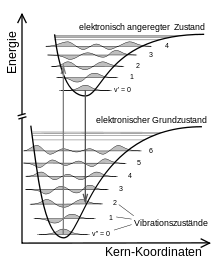
\includegraphics[width=5cm]{Fluoreszenz_Energie_Graph_elektronische_Zustaende.png}
	\label{fig:Energiegraphen der elektronischen Zustände bei der Fluoreszenz}
	\caption{Potentialkurven zweier elektronischer Zustände in Abhängigkeit des Kernabstandes in einem fluoreszierenden System \cite{wikiFranckCondonPrinzip}.}
\end{dsafigure}

Nach dem Franck-Condon-Prinzip gilt, dass der Übergang zwischen elektronischen Zuständen so verläuft, dass die Kernwellenfunktionen einen maximalen Überlapp haben. Zudem wird angenommen, dass die Anregung (und Bewegung der Elektronen) so schnell abläuft, dass die Kernbewegung ignoriert werden kann. Atomkerne sind rund 2000-mal schwerer als Elektronen und bewegen sich daher oft entsprechend langsamer. In Abbildung \ref{fig:Energiegraphen der elektronischen Zustände bei der Fluoreszenz} kann man sehen, dass die Pfeile als Darstellung für den Übergang vertikal verlaufen. Beschrieben wird dies durch die Franck-Condon-Näherung, die unter anderem besagt, dass die Wahrscheinlichkeit der Emission dort am höchsten ist, wo die Kernwellenfunkionen den größten Überlapp haben (siehe Abbildung \ref{fig:Energiegraphen der elektronischen Zustände bei der Fluoreszenz}).
